\documentclass[ebook,11pt]{memoir}
%\areaset[0.375in]{4.5in}{8in} % Matches this http://tex.stackexchange.com/questions/19497/how-do-you-setup-a-tex-document-to-self-publish-a-book-online
%openany prevents chapters from starting a new right page with a bunch
%of blank pages, but still doesn't do what I want exactly

\renewcommand{\thechapter}{\Roman{chapter}}
\chapterstyle{thatcher}

\usepackage[obeyFinal,final]{todonotes}
%\usepackage[draft]{todonotes}
\usepackage[lining,scaled=.95]{ebgaramond}
\usepackage[T1]{fontenc}
\usepackage{graphicx}

\aliaspagestyle{part}{empty}
%\setsecnumdepth{none}
%\maxsecnumdepth{none}

\copypagestyle{modruled}{ruled}
\makeevenhead{modruled}{}{\scshape Lev Tolstoy}{}
\makeoddhead{modruled}{}{\scshape Childhood}{}
\makeevenfoot{modruled}{}{\thepage}{}
\makeoddfoot{modruled}{}{\thepage}{}

\addtopsmarks{modruled}{}{%
% \renewcommand\partmark[1]{\markboth{\partname \thepart. #1}}
  \renewcommand\chaptermark[1]{}
  \renewcommand\sectionmark[1]{}
}

% hyphenation rules
\hyphenation{Ivan-ych StackExchange deft-ly quick-ly}

%\includeonly{preface}

\begin{document}

\frontmatter

\newlength{\drop}\setlength{\drop}{0.12\textheight}

\newcommand*{\firsttitle}{\begingroup
\centering
\vspace*{3em}
{\Large CHILDHOOD}\\[\baselineskip]
{\Large LEV NIKOLAYEVICH TOLSTOY}
\vfill\null
\endgroup}

% Adapted from Peter Wilson's _Some Examples of Title Pages_, 2010.
\newcommand*{\titleAM}{\begingroup
\centering
\vspace*{\drop}
{\large Lev Nikolayevich Tolstoy}\\[\baselineskip]
{\Huge CHILDHOOD}\\[\baselineskip]
%{\Huge ADOLESCENCE,}\\[\baselineskip]
%{\Huge YOUTH}\\[\baselineskip]
{\scshape translated from the russian}\\
{\scshape by}\\
{\scshape chris tessone}\\
\vfill%[10.0\baselineskip]
{\scshape 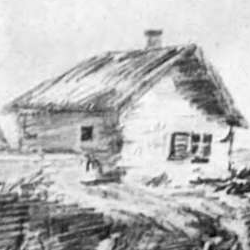
\includegraphics[width=1.5cm, height=1.5cm]{taman-press.png}}\\[0.5\baselineskip]
{\small\scshape the taman press}\par
{\small Silver Spring, Maryland}\par
{\small\scshape 2015}\par
\endgroup}

\firsttitle
\thispagestyle{empty}
\clearpage

\newpage\null\thispagestyle{empty}\newpage

\titleAM
\thispagestyle{empty}
\clearpage 


%\maketitle
%\thispagestyle{empty}
%\clearpage 

\begingroup 
\footnotesize 
\parindent 0pt 
\parskip \baselineskip 
Copyright \textcopyright{} 2015 Christopher A.~Tessone \\
All rights reserved \\
Printed in the United States of America %% true of Lulu, is it true 
                                %% of others?

This work will someday be placed under a more permissive license. For 
now, please email me at chris@tessone.net if you want to do anything 
with this document. 

Typeset in \LaTeX\ with much-appreciated assistance from the \TeX\
community on StackExchange. %% provide font information 

%%\textit{Library of Congress Cataloging-in-Publication Data} %% http://www.loc.gov/publish/cip/

Lev Nikolayevich Tolstoy, 1828--1910, author. \\
$[$Category information. English.$]$ \\
Childhood, Adolescence, Youth / Lev Tolstoy ; translated by Chris 
Tessone. \\
More to follow. 

\vfill 

Publisher Information\\
Publisher Address\\
Email or web presence 

\endgroup 
\pagestyle{empty}
\clearpage 


\pagestyle{modruled}

\mainmatter

\newpage
\thispagestyle{empty}
\mbox{}
\part*{Childhood}
\makeoddhead{modruled}{}{\scshape Childhood}{}
\markboth{Childhood}{}

\chapter{Karl Ivanych, the Tutor}

On the 12th of August, 18\ldots{}, exactly the third day after my birthday, when I turned ten and received such marvelous gifts, Karl Ivanych woke me up at seven o'clock in the morning, hitting the wall just above my head with a flyswatter made from sugar paper and a stick. He did this so carelessly that he hit the icon of my angel\todo{that is, patron saint---footnote needed}, which was hanging from the oak headboard, and the dead fly fell right on my head. I stuck my nose out from under the cover, stopped the icon, which was still swinging, with my hand, knocked the dead fly onto the floor, and threw an angry look at Karl Ivanych, my eyes still clouded with sleep. He was wearing a motley cotton dressing-gown, belted with a belt from the same material, a red knit cap with a tassel, and soft goat-skin \todo{?} boots, and he continued to walk along the walls, looking for targets and slapping with his flyswatter.

``Fine,'' I thought, ``I \emph{am} small, but why does he keep bothering me? Why doesn't he swat flies by Volodya's bed? There are so many over there! No, Volodya is older than me; I'm the youngest: that's why it's me he torments. That's what he thinks about all day,'' I whispered, ``how to make trouble for me. He can see very well that he woke me up and frightened me, but he acts like he doesn't notice\ldots{} what a disgusting person! His robe, his little hat, and that tassel---disgusting!'' %narr

At the same time I was mentally expressing my annoyance with Karl Ivanych, he went over to his bed, looked at his watch, which was hanging over it in a beaded slipper, hung the flyswatter up on its nail, and, obviously in a very pleasant mood, turned to us.

\textit{``Auf, Kinder, auf!\ldots{} s'ist Zeit. Die Mutter ist schon im Saal,''} he shouted in his kind German voice, then he went over to me, sat by my feet, and took his snuff box out of his pocket.\footnote{Up, children, up! 'Tis time. Mother is already in the hall. \textit{(Ger.)}} I pretended I was still sleeping. Karl Ivanych took snuff, wiped his nose, snapped his fingers, and then started in on me. Laughing, he started to tickle the soles of my feet. \textit{``Nu, nun, Faulenzer,''} he said.\footnote{Well, now, lazy boy! \textit{(Ger.)}} %karl

However much I dreaded the tickling, I did not jump out of bed and did not answer him, instead hiding my head deeper under the pillows, kicking my feet as hard as I could and doing everything I could to keep from laughing.

``He's so kind and loves us so much, and I was thinking such awful things about him!'' %narr

I was annoyed both at myself and at Karl Ivanych, wanting to laugh and wanting to cry: my nerves were unsettled.

\textit{``Ach, lassen sie, Karl Ivanych!''}~I shouted with tears in my eyes, sticking my head out from under the pillows.\footnote{Leave me alone, Karl Ivanych! \textit{(Ger.)}} %narr

Karl Ivanych seemed surprised, left the soles of my feet in peace, and started asking with concern: what was it? had I had a nightmare?\ldots{} his kind German face and the sympathy with which he tried to guess the reason for my tears made them flow all the more abundantly: I was ashamed, and I could not understand how just a minute before I could not love Karl Ivanych and find his robe, hat, and tassel so disgusting; now, on the contrary, all of this seemed extremely endearing, and even the tassel seemed like a clear indication of his kindness. I told him that I was crying because I had had a nightmare---as if maman had died and they were taking her to the grave.\footnote{Tolstoy uses French \textit{papa} and \textit{maman} throughout for the narrator's parents. Because they are used so extensively, I have left them untranslated but also in normal script rather than italicizing them. --- Trans.} I made all this up, because I absolutely could not remember what I had dreamed about that night; but when Karl Ivanych, touched by my story, started to comfort and soothe me, I started thinking I had indeed had that nightmare, and my tears started flowing for another reason. 

When Karl Ivanych left me, and I, sitting up a little in bed, started to pull my stockings \todo{?} onto my little legs, my tears had subsided a little, but the dark thoughts brought on by my imagined dream did not leave me. Uncle \todo{need a footnote...} Nikolai came in---a small, neat little man, always serious, exact, respectable, \todo{?} and a great friend of Karl Ivanych. He brought our dresses and shoes: boots for Volodya, for me still an intolerable pair of children's shoes with bows. \todo{specific term for shoes?} I was ashamed to cry in front of him; the morning sun was shining through the window besides, and Volodya, mimicking Marya Ivanovna (our sisters' governess), was laughing so happily and sonorously, standing over the wash stand, that even serious old Nikolai, a towel over his shoulder, with soap in one hand and a basin in the other, smiling, said:

``That's enough, Vladimir Petrovich, kindly wash up.'' %unclenikolai

I cheered up completely.

\textit{``Sind sie bald fertig?''} Karl Ivanych's voice came from the classroom.\footnote{Are you almost ready? \textit{(Ger.)}} %karl

His voice was strict and no longer had the same tone of kindness that had touched me and brought me to tears. In the classroom, Karl Ivanych was an entirely different person: he was a schoolmaster. I dressed quickly, washed up, and, with a brush in my hand, smoothing my wet hair, I answered his call.

Karl Ivanych, with glasses on his nose and a book in his hand, sat in his usual place, between the door and the window. To the left of the door were two little shelves: one was ours, the children's, the other was Karl Ivanych's, his \emph{personal} shelf. On ours were all sorts of books---educational and non-educational: some were standing up, others were lying down. Only the two large volumes of \textit{Histoire des voyages} in red covers rested sedately against the wall;\footnote{History of the Voyages. \textit{(Fr.)}} \todo{Voltaire?} then there were long, thick, large, and small books---covers without books and books without covers; we used to push and shove them in there before recess, when we were told to put the library, as Karl Ivanych loudly called that shelf, in order. The collection of books on his \emph{personal} shelf, if not so large as the one on ours, was even more varied in composition. From those books, I remember three: a German brochure on the manuring of cabbage gardens---without a cover, one volume containing a history of the Seven Years' War---in parchment, burnt at one corner, and a full course on hydrostatics. Karl Ivanych spent the greater part of his time reading, even ruining his eyes in the process; but other than those books and the \textit{Northern Bee}, he read nothing else.

Among the items lying on Karl Ivanych's shelf, I am constantly reminded of one in particular. It was a little circle of cardboard, set on a wooden base to which the cardboard circle was attached by way of a few pins. On this circle, a picture was pasted, a caricature of a lady and a hairdresser. Karl Ivanych was very good at pasting things together and had devised the circle himself and made it to protect his weak eyes from bright light.\todo{Run on ok?}

I can see him before me now a long figure in a cotton dressing-gown with sparse grey hair sticking out from his little red hat. He sits by a little table, on which the circle with the hairdresser is standing, casting a shadow over his face; in one hand he holds a book, the other rests on the arm of the chair; near him lies his watch, with a painted hunter on the dial, a checkered handkerchief, a round black snuff box; a green eyeglass case, a set of tongs on a tray. \todo{I think this is right, not translated by the Maudes!} Every item was so sedately, so exactly placed that by their good order alone one could conclude that Karl Ivanych's conscience was clean and his soul at peace.

At times, after we had had enough of running around downstairs in the hall, I would sneak up to the classroom on tiptoe---Karl Ivanych would be sitting there alone in his chair, reading one of his favorite books with a peaceful and sublime expression. Sometimes I would find him in a moment when he was not reading: his glasses would be at the very end of his aquiline nose, his blue eyes, half-closed, would be staring off into the distance with a peculiar gaze, and his lips would be smiling sadly. It would be quiet; the only sounds would be his even breathing and the ticking of his watch with the hunter.

At times he would not notice me, and I would stand at the door and think: poor, poor old man! There are so many of us, we are playing, we are enjoying ourselves, and he is all by his lonesome, \todo{neologism, ok?} and he has no one to show him affection. It is true what he says, that he is an orphan. And the story of his life is so terrible! I remember when he told it to Nikolai---it would be terrible to be in his position! And I feel such pity for him that I would at times come up to him, grab his hand, and say, \textit{``Lieber Karl Ivanych!''} He loved it when I talked to him like that; he would always look at me with affection, and I could tell that he was deeply moved.

On the second wall hung maps, nearly all of them tattered, but skillfully mended by Karl Ivanych's hand. On the third wall, in the middle of which was the door leading downstairs, on one side hung two rulers: one, ragged, was ours, the other, a new one, was his \emph{personal} ruler, used more for discipline than for drawing lines; on the other side was a blackboard on which our serious offences were marked with circles and our minor ones with little crosses. To the left of the board was a corner, where they made us kneel.

How I remember that corner! I remember the flap of the stove, the vent in that flap, and the noise that it made when you moved it. At times I would be kneeling there in the corner, kneeling, kneeling, so that my knees and back hurt, and I would think: Karl Ivanych has forgotten about me: I suppose he is sitting there peacefully in his soft chair and reading his hydrostatics---and what about me? And I would start to open and shut the vent or pick plaster off from the wall; but if too large a piece suddenly fell on the ground with a loud noise, well, the fear alone was worse than any punishment. I would glance over at Karl Ivanych---and he would be sitting quietly with a book in his hand, as if he had not noticed a thing.

In the middle of the room stood a table covered with ragged oilcloth, the corners visible underneath ragged with the cuts of our pen knives. Around the table were a few stools, unfinished but worn smooth from long use. The final wall was taken up by three little windows. This was the view from them: right under the windows was a road, every potholes, every pebble, every rut of which was long since known and dear to me; beyond the road was a little park full of trimmed lilac, behind which a wicker fence could be seen; through the trees, a meadow was visible, with a barn to one side of that and the forest opposite; far away in the forest, the warden's little hut was visible. From the window, to the right, part of the terrace was visible, where the grown-ups would usually sit until dinner. At times, while Karl Ivanych was correcting our dictation, I would look out that side, see mother's black hair, someone's back, and hear vague conversations and laughter from there; then I would get annoyed that I could not be there and think: \textit{when will I be a grown-up, stop studying, and be able to sit with the people I love instead of doing dialogues?} My annoyance would turn into sadness and, God knows why, or what I was thinking about, but I would not hear a word of Karl Ivanych, who was angry about my mistakes. %narr

Karl Ivanych took off his robe, put on his blue tail coat with pleats and folds \todo{?} on the shoulders, straightened his tie in front of the mirror, and guided us downstairs to say good morning to mother.

\chapter{Maman}

Mother sat in the drawing room and was pouring tea; with one hand she held the teapot, and with the other the tap of the samovar, from which water was flowing through the top of the teapot and onto the tray. But although she was staring intently, she did not notice this, nor did she notice that we had come in.

So many memories of the past surface when you try to resurrect features of a loved one that you can see them only vaguely through those memories, clouding your vision like tears. Those are tears of the imagination. When I try to remember mother as she was at that time, I see only her brown eyes, which always expressed kindness and love equally, the mole on her neck, a little below the place where her little curly hairs began, her embroidered white collar, her dry, tender hand, which caressed me so often and which I often kissed; but the overall picture slips eludes me.

To the left of the sofa stood an old English piano; in front of the piano sat my dark-looking sister, Lyubochka, her pink fingers, just washed with cold water, playing Clementi's etudes with visible effort. She was eleven years old; she went around in a short linen dress and white, lace-trimmed pants and could manage octaves only in arpeggio. Near her, half-turned away, sat Marya Ivanovna in a bonnet with pink ribbons, in a light blue caraco jacket and with a red, angry face, which took on an even stricter expression as soon as Karl Ivanych walked in. She looked at him menacingly and, not answering his bow, continued, tapping her foot, to count: \textit{un, deux, trois, un, deux, trois} louder and more demandingly than before.

Karl Ivanych, not paying even the slightest attention to this, as usual, went directly to mother's hand with a German greeting. She came to her senses, shook her head, as if by this gesture trying to drive away unpleasant thoughts, gave her hand to Karl Ivanych and kissed him on his wrinkled temple, at the same time he kissed her hand:

\textit{``Ich danke, lieber Karl Ivanych,''} and, continuing to speak in German, she asked:\footnote{My thanks, dear Karl Ivanych. \textit{(Ger.)}} %maman

``Did the children sleep well?'' %maman

Karl Ivanych was deaf in one ear, and now, because of the noise from the piano, he could hear nothing at all. He stooped closer to the sofa, leaned with one arm on the table, supporting himself with one leg, and, with a smile that seemed to me the height of sophistication, lifted his hat a little off his head and said:

``You will forgive me, Natalya Nikolayevna?'' %karl

Karl Ivanych, so that his bare head did not catch cold, never took off his little red hat, but he asked forgiveness for this each time he came into the drawing room.

``Put it back on, Karl Ivanych\ldots{} I am asking you, did the children sleep well?'' asked maman fairly loudly, moving closer to him. %maman

But he again heard nothing, covered his bald spot with the little red hat, and smiled even more sweetly.

``Stop for a minute, Mimi,'' said maman to Marya Ivanovna with a smile: ``we can't hear anything.'' %maman

When mother smiled, though her face was already pretty, she became incomparably more beautiful, and everything around her seemed to become brighter. If in the heaviest moments of my life I could have just caught a glimpse of that smile, then I would never have known what sorrow is. It seems to me that the smile alone holds what we call beauty: if a smile adds charm to a face, then the face is very fine; if it does not change, then it is ordinary; and if it ruins the face, then it is ugly.

Having greeted me, maman took my head in both hands and leaned it back, then looked at me fixedly and said:

``Did you cry today?'' %maman

I did not answer. She kissed my eyes and asked in German:

``What were you crying about?'' %maman

When she talked with me in this friendly way, she always spoke in that language, which she had mastered to perfection.

``It was a dream, maman, that's why I was crying,'' I said, remembering in all its detail my made-up dream and shuddering involuntarily at the thought. %narr

Karl Ivanych confirmed my words but was silent about the dream. Changing the subject to the weather---a conversation which Mimi also took part in---maman put six pieces of sugar for some of the more valued servants, stood up and went over to the lace frame that stood by the window.

``Well, go to papa now, children, and tell him he needs to come see me before he goes out to the barn.'' %maman

The music, the counting, and the menacing glances began again, and we went to papa. Walking through another room, which from my grandfather's days was still called the footman's pantry, we went into his study.

\chapter{Papa}

He was standing by his desk and, pointing at some envelopes, papers, and piles of money, speaking heatedly, and explaining something angrily to the steward, Yakov Mikhaylov, who was standing in his usual place between the door and the barometer, his hands placed behind his back, and was quickly moving his fingers back and forth.

The angrier papa got, the faster the fingers moved: likewise, when papa stopped, the fingers stopped as well; but when Yakov himself started talking, the fingers became extremely agitated and flew around desperately in every direction. It seemed to me that one could guess Yakov's secret thoughts by their movements; his face was always calm---it expressed an awareness of the merits of his case, but also of his subordinate position, in other words: I am right, however, as you like it!

Seeing us, papa merely said:

``Wait, just a moment.'' %papa

And he nodded his head at the door, so that one of us would shut it.

``Oh, merciful heavens! What is with you today, Yakov?'' he continued saying to the steward, twitching his shoulder (he had a habit of doing that). ``This envelope, with 800 rubles enclosed\ldots{}'' %papa

Yakov moved beads on the counting frame, sliding over 800, and turned his gaze on some indeterminate point, waiting for what would come next.

``\ldots{} for housekeeping expenses in my absence. Understand? You should get 1,000 rubles from the mill\ldots{} Yes or no? You should get 8,000 back from the Treasury bonds; by your estimates we can sell 7,000 pounds of hay---I will put it out for 45 kopecks---so you should get 3,000; so how much money do you get in the end? 12,000\ldots{} Yes or no?'' %papa

``Yes, exactly, sir,'' said Yakov. %yakov

But from the quickness with which his fingers moved, I could tell he wanted to object; papa stopped him:

``Well, from that money you will send 10,000 to the Council for Petrovskoye. Then the money that is at the bank,'' continued papa, while Yakov mixed up the count and put up 21,000 instead of 12,000, ``you will bring to me and show as an expense as of this date.'' Yakov mixed up the count and turned over the counting-frame, apparently showing by this movement that the 21,000 would be spent. ``This envelope with the money you will send in my name to the address listed.'' %yakov

I was standing close to the desk and looked at the inscription. On the envelope was written: ``To Karl Ivanovich Mauer.''

Apparently noticing that I had read something that I did not need to see, papa put his hand on my shoulder and with an easy movement showed me away from the desk. I did not know whether it was a caress or a reproach; in any case, I kissed the large, sinewy hand that was lying on my shoulder.

``Yes, sir,'' said Yakov. ``And what orders are there for the Khaborovka money?'' %yakov

Khabarovka was mother's village.

``Leave it in the bank and do not use them for anything, under any circumstances, without my orders.'' %papa

Yakov was silent for a few seconds; then suddenly his fingers began to whirl around with double the speed, and he, changing his expression from the one of dull obedience with which he listened to his master's orders to his more characteristic expression of sharp cunning, moved the counting frame toward him and began to speak:

``Permit me to report, Pyotr Aleksandrych, that it will not be possible to pay even the Council on time as you wish. You were so kind as to say,'' he continued after a pause, ``that we should receive money from the bonds, from the mill, and from the hay\ldots{}'' Counting out all of these items, he slid beads over to show each one. ``But I am afraid we may be mistaken in our estimates,'' he added, falling silent for a while and looking gravely at papa. %yakov

``Why?'' %papa

``If you would be so kind as to see: regarding the mill, the miller has come to me twice already to ask for a deferment and swore by Christ our Lord that he did not have the money\ldots{} And he is actually here now: perhaps you would like to speak with him yourself?'' %yakov

``What does he have to say?'' asked papa, shaking his head to show that he did not want to speak with the miller. %papa

``Isn't it clear? He says there was nothing to mill, and what little money there was, he had to put it all into the dam. So, if we take him off the mill, \emph{sir}, do you think we will make our estimates then? You were so kind as to speak about the bonds, well, I believe I already reported to you that once we put our money in them, we could not get it back soon. The other day, I sent a cart of flour to Ivan Afanasyich in the city, along with a note about this matter: he answered the same as before, I am happy to make an effort for Pyotr Aleksandrych, but the matter is not in my hands, and that everything suggests it will be two months or more until our check comes. You were so kind as to speak about the hay, let us assume that it can sell for 3,000\ldots{}'' %yakov

He slid 3,000 over on the counting frame and was silent for a minute, looking first at the counting frame, then into papa's eyes, with an expression that said:

``You can see for yourself how little this is! And we'll take a loss on the hay in any case if we sell it right now, you know that yourself\ldots{}'' %yakov

It was clear that had a large reserve of such arguments left; it must have been for this reason that papa interrupted him.

``I am not going to change my orders,'' he said, ``but if there is, in fact, any delay in receiving this money, then there's nothing that can be done, take whatever is needed from the Khaborovka money.'' %papa

``Yes, sir.'' %yakov

By Yakov's fingers and the expression on his face, it was obvious that this last order gave him great pleasure.

Yakov was a serf, an extremely diligent and devoted person; like all good stewards, he was tightfisted in the extreme on his master's behalf and had the strangest conceptions about his master's interests. He was perpetually looking after profit for his master's estate at the expense of his mistress's estate, always trying to prove that it was unavoidable to spend the revenues from her property on Petrovskoye (the village in which we lived). At the present moment, he was triumphant, because he had succeeded perfectly in this.

Having greeted us, papa told us what lazybones we had become out in the country, that we were no longer little, and that it was time for us to study seriously.

``You already know, I think, that I am going to Moscow tonight, and I am taking you with me,'' he said. ``You are going to live at your grandmother's, and maman and the girls will stay here. And you know that only one thing will make me pleased---and that is to hear that you are studying hard and that they are satisfied with you there.'' %papa

Although the preparations that had been obvious for a few days had prepared us for something unusual to happen, this news nevertheless affected us terribly. Volodya turned red and with a quivering voice gave him mother's message.

``Then this is what my dream was predicting!'' I thought. ``Please God, don't let anything worse happen.'' %narr

I was very, very sad for mother, but, at the same time, the thought that we had become grownups made me happy.

``If we are going today, then surely there won't be any classes: that is nice!'' I thought. ``But I am sad for Karl Ivanych. They will probably let him go, or else they wouldn't have made that envelope for him\ldots{} It would be better to have to study for a century but not go away, not leave mother behind, and not treat poor Karl Ivanych so badly. He is already so unhappy!'' %narr

These thoughts flashed through my head; I did not move from the spot and looked fixedly at the black bows on my shoes.

Having said a few words with Karl Ivanych about the falling barometer and having ordered Yakov not to feed the dogs, so he could ride out after dinner on a fairwell hunt with the young hounds, papa, against my expectations, sent us to study, consoling us, however, with a promise to take us on the hunt.

On the way upstairs I ran out onto the terrace. Near the doors, lying in the son and squinting her eyes, lay father's favorite borzoi dog, Milka.

``Milochka,'' I said, caressing her and kissing her snout, ``we are going today; goodbye! We'll never see each other again.'' %narr

I was deeply affected by this and cried.

\chapter{Classes}

Karl Ivanych was already in a bad mood. This was obvious from his furrowed brow, and from the way he had thrown his frock coat in the bureau, \todo{?} and how he angrily belted up his robe, and how forcefully he had dug his nail into the place in the dialogue book where the passage that we were supposed to memorize ended. Volodya made a decent effort at studying; I, on the other hand, was so upset that I could not do anything at all. For a long time, I sat gazing senselessly at the dialogue book, but because of the tears welling up in my eyes at the thought of our imminent parting, I could not read; when the time came for me to repeat them to Karl Ivanych, who, squinting, listened to me (this was a bad sign), I came to the place where one person says, \textit{``Wo kommen sie her?''} and the other answers: \textit{``ich komme vom Kaffe-Hause,''} and I could not hold back my tears any longer, unable because of my sobbing to pronounce the words: \textit{``Haben sie die Zeitung nicht gelesen?''}\footnote{Where are you coming from? I am coming from the cafe. Have you read the newspaper? \textit{(Ger.)}} When we turned to penmanship, I left so many blots on the page because of the tears that I let fall that it was like I was writing with water on parcel paper.

Karl Ivanych got angry, made me kneel in the corner, said over and over that I was being obstinate, that I was playing a farce (this was his favorite phrase), threatened me with the ruler, and demanded that I ask his pardon when I could barely get out a word for crying; finally, seemingly feeling the injustice of what he was doing, he went into Nikolai's room and slammed the door.

From the classroom, I could hear the conversation in Uncle Nikolai's room.

``You heard, Nikolai, that the children go to Moscow?'' said Karl Ivanych, entering the room. %karl

``I heard, of course.'' %unclenikolai

Nikolai must have been about to stand up, because Karl Ivanych said, ``Sit, Nikolai!'' and right after that shut the door. I came out of the corner and went over to the door to eavesdrop.

``No matter what kind things you do to people, no matter how attached you are, you obviously cannot be expecting gratitude, eh, Nikolai?'' said Karl Ivanych with feeling. %karl

Nikolai, sitting by the window, repairing shoes, nodded his head.

``I am living in this house twelve years and can say before God, Nikolai,'' continued Karl Ivanych, lifting his eyes and his snuff box toward the ceiling, ``that I have loved them and helped them more than as if they were my own children. You remember, Nikolai, when Volodyenka had the fever, you remember how I sat for nine days by his bed, not closing my eyes. Yes: then I was nice, kind Karl Ivanych, then I was needed; but now,'' he added, smiling ironically. ``Now \emph{the children have become grown ups: they need to study seriously.} As if they don't study anything here, right, Nikolai?'' %karl

``Of course they do,'' said Nikolai, putting down his stitching awl and spreading out the thread with both hands. %unclenikolai

``Well, now I have become not needed, they need to throw me out; and where are the promises? where is the gratitude? I love and respect Natalya Nikolayevna, Nikolai,'' he said, placing his hand on his chest, ``but what does she have to do with it\ldots{}? They don't care about her desires in this house, that's it.'' At this he threw a scrap of leather onto the floor with a significant gesture. ``I know whose tricks these are and why I have become not needed: because I am not always flattering and conniving like \emph{some people}. I am used to always and in front of everyone telling the truth,'' he said proudly. ``Forget about them, for God's sake! They are not getting any richer because I will not be here, and I will find my bite of bread, if God is merciful\ldots{} Don't you think, Nikolai?'' %karl

Nikolai lifted his head and looked at Karl Ivanych as if to ascertain whether he really could find his bite of bread---but he said nothing.

Karl Ivanych went on in this vein for a long time: he talked about how they knew how to value his services much better in some general's house where he lived before (it was very painful for me to hear that), talked about Saxony, about his parents, about his friend, the tailor Sch\"onheit, etc., etc.

I empathized with him in his sorrow, and it pained me that father and Karl Ivanych, whom I loved almost equally, did not understand one another; I again went into the corner, got down on my knees, and debated with myself about how to re-establish harmony between them.

Returning to the classroom, Karl Ivanych told me to stand up and prepare my notebook for writing from dictation. When everything was ready, he lowered himself majestically into his chair and, in a voice that seemed to come from a great depth, began to dictate the following: \textit{``Von al-len Lei-den-schaf-ten die grau-samste ist\ldots{} haben sie geschrieben?''}\footnote{Of all the passions, the cruelest is\ldots{} Have you written that? \textit{(Ger.)}} Here he stopped, slowly took snuff, and continued with new strength: \textit{``die grausamste ist die Un-dank-bar-keit\ldots{}''}\footnote{The cruelest is Ingratitude\ldots{} Capital I. \textit{(Ger.)}} Waiting for the continuation, having written the last word, I looked at him. %karl

\textit{``Punctum,''} he said with a barely noticeable smile and gestured for us to give him our notebooks.\footnote{Period. \textit{(Lat.)}} %karl

He read this aphorism several times with different intonations and with an expression of the greatest pleasure, expressing as it did his mostly deeply felt thought; then he gave us a history lesson and sat down by the window. His face was not sullen as before; it expressed the contentment of a person who had suitably avenged himself for a wrong imposed on him.

It was a quarter till the hour; but Karl Ivanych, it seemed, was not thinking about letting us go: he was constantly giving us new lessons. Boredom and our appetites increased in equal measure. With the greatest impatience I followed the signs that suggested dinner was near. First a servant girl with a washcloth coming to wash the plates, then the sound of dishes in the dining room, the table being moved and the chairs begin dragged into place, then Mimi with Lyubochka and Katyenka (Katyenka was Mimi's twelve year old daughter) coming in from the garden; but Foka was nowhere to be seen---Foka, the butler, who always came in and announced that the food was ready. Only then could we throw down our books and, paying no attention to Karl Ivanych, run downstairs.

Just then we heard steps on the stairs; but it was not Foka! I had learned his gait and could always recognize the creaking of his boots. The door opened, and a figure appeared that was completely unknown to me.

\chapter{The Holy Fool}

A man of about fifty entered the room; he had a pale, pockmarked, elongated face, long, grey hair, and a sparse, reddish beard. He was so tall that, in order to pass through the door, he not only had to bend his head down but bend at the waist as well. He wore something tattered that looked like a kaftan worn over a cassock; in his hand, he held an enormous staff.\footnote{The Russian kaftan was a coat or gown with long sleeves and a high collar, which buttoned down the front, very different from the garments that go by the name in other countries. --- Trans.} Entering the room, he knocked on the floor as hard as he could with it, and, his brows crooked and his mouth open outrageously wide, he roared with the most frightening and unnatural laughter. One of his eyes was crooked, and the white pupil of that eye danced incessantly and gave his already unattractive face an even more disgusting \todo{?} appearance.

``Aha! You're caught!'' he cried, running up to Volodya with short little steps, and grabbed him by the head, thoroughly inspecting it---then, with a perfectly serious expression he stepped back, went up to the table, and began to blow under the oilcloth and make the sign of the cross. ``Oh, misery! Oh, pain\ldots{}! My dearest ones\ldots{} they're flying away,'' he said, his voice trembling from tears, looking passionately and intently at Volodya, and started to wipe away his tears, which were indeed falling, with his sleeve. %grisha

His voice was hoarse and rough, his movements hurried and erratic, his speech nonsensical and rambling (he never used pronouns), but the cadence was so affecting, and his yellow, deformed face sometimes took on such an open, sorrowful expression, that, listening to him, it was impossible not to feel a mixture of pity, fear, and grief.

This was Grisha, a holy fool and pilgrim.

Where was he from? Who were his parents? What compelled him to choose the pilgrim's life that he led? No one knew. All I know is that since 1815 \todo{?} he was known as a holy fool, who winter and summer went around barefoot, visiting monasteries, giving little images of saints \todo{better than icons?} to those he came to love, and saying mysterious things, which some people took as prophecies, that no one had ever known him in any other condition, that every now and then he would go to see grandmother, and that some said he was the unhappy son of rich parents and was pure of spirit, while others said he was just a peasant and an idler.

Finally, the long awaited and punctual Foka appeared, and we went downstairs. Grisha, sobbing and continuing to speak all kinds of absurdities, came after us and knocking his crutch against the steps of the stairs. Papa and maman were walking around the drawing room arm-in-arm and talking quietly about something. Marya Ivanovna sat sedately on one of the chairs that were arranged symmetrically at right angles to the sofa, and, with a strict but restrained voice gave instruction to the girls, who were next to her. \todo{look over that sentence again} As soon as Karl Ivanych entered the room, she looked at him and immediately turned away, and her face took on an expression that can be described as saying: I do not notice you, Karl Ivanych. By the girls' eyes it was obvious that they wanted badly to give us some very important piece of news; but to jump up from their places and go over to us would have been a violation of Mimi's rules. We first had to go over to her, say, ``Bonjour, Mimi!'' \todo{punct.} shuffle our feet, and only then were we allowed to enter into conversations.

What an intolerable individual that Mimi was! It always seemed that no topic was permissible around her: she found everything indecent. On top of that, she was forever nagging us: \textit{``parlez donc fran\c cais,''} and it was our bad luck that dinner was precisely where we wanted to chatter away in Russian; and just as you were digging into a dish and wanted to be left alone, then, without fail, it would be, \textit{``mangez donc avec du pain,''} or, \textit{``comment ce que vous tenez votre fourchette?''}\footnote{Speak French \ldots{} eat with bread \ldots{} how are you holding your fork? \textit{Fr.}} \todo{Added graf break here, not in original.} %mimi

\textit{What business is it of hers?} I would think. \textit{Let her teach her girls, we have Karl Ivanych for that.} I shared his hatred for \emph{some people} completely. 

``Ask mama if you can take us along on the hunt,'' said Katyenka in a whisper, pulling on my jacket to stop me as the grown-ups were going ahead into the dining room. %katyenka

``Alright, we'll try.'' %nikolai

Grisha ate in the dining room, but at a special little table; he did not raise his eyes from his plate, sighed from time to time, made frightening faces, and said, as if talking to himself, ``A pity! She flew away\ldots{} The dove will fly away into the heavens\ldots{} oh, the stone on the grave!'' and so on. %grisha

Maman had been out of sorts since morning; Grisha's words and actions noticeably deepened her sad disposition. 

``Oh, yes, I almost forgot to ask you about one thing,'' she said, handing father a dish filled with soup. %maman

``What was it?'' %papa

``Tell them to lock up your frightening dogs, please; they very nearly bit poor Grisha when he came through the yard. They could attack the children, too.'' %maman

Hearing that they were talking about him, Grisha turned to the table, started showing everyone the tattered ends of his clothes, and said, while chewing:

``Wanted them to tear me to pieces\ldots{} God would not allow it. A sin to let the dogs torment me! A great sin! Don't beat the big man,\footnote{He called all men this, without distinction. --- \textit{LNT.}} what's a beating? God forgives\ldots{} Not in these days.'' %grisha

``What is he saying?'' asked papa, examining him with a fixed and severe gaze. ``I don't understand anything.'' %papa

``I understand him,'' answered maman: ``He told me that some hunter set his dogs on him on purpose, so he's saying, `He wanted them to tear me to pieces, but God would not allow it, and asks you not to punish him for it.''' %maman

``Ah! So that's it!'' said papa. ``How does he know that I want to punish that hunter?'' He then continued in French: ``You know that I am not very enthusiastic about these holy men, but that one especially bothers me, and he ought to\ldots{}'' %papa

``Ah, don't say that, my friend,'' maman interrupted him, as if frightened by something, ``what could you know about him?'' %maman

``Well, I suppose I've had the chance to study their sort of people---so many of them come to you---they're all alike. Always the same story\ldots{}'' %papa

It was clear that mother had an entirely different opinion about that and did not want to argue.

``Pass me that pie, please,'' she said. ``Well, are things going well today?'' %maman

``No, it makes me angry,'' papa continued, picking up the pie, but holding it at such a distance that maman could not reach it, ``no, it makes me angry when I see intelligent and educated people being taken in by lies.'' %papa

And he struck the table with his fork.

``I asked you to pass me the pie,'' she repeated, reaching out her hand.

``And it is wonderful,'' continued papa, moving his hand away, ``that the people like that get picked up by the police. The only good they do is upset the weak nerves of certain individuals,'' he added with a smile, noting that the conversation was bothering mother a great deal, and gave her the pie.

``I'll say only this: it's difficult to believe that a person who, in spite of his sixty years, walks around winter and summer barefoot and wears seventy pounds of chains under his clothing, never taking them off, and who more than once has turned down offers to live peacefully with all his needs met---it's difficult to believe that a person would do all of that just out of laziness.'' %maman

``Concerning the prophecies,'' she added with a sigh, falling silent for a moment, ``\textit{je suis pay\'ee pour y croire};\footnote{I have paid to be believed. \textit{Fr.}} \todo{check this French translation.} I'm sure I've told you how Kiryusha prophesied my late papa's death to the day and the hour.'' %maman

``Ah, what have you done to me!'' said papa, smiling and placing his hand by his mouth on the side where Mimi was sitting. (When he did this, I always listened with rapt attention, expecting something funny.) ``Why did you remind me of his feet? I just looked at them and now I won't eat anything.'' %papa

Dinner was coming to an end. Lyubochka and Katyenka were winking at us incessantly, turning in their chairs, and generally expressing serious agitation. Their winking meant: ``why aren't you asking if you can take us along on the hunt?'' I jabbed Volodya with my elbow, Volodya jabbed back, and finally we decided: first with a timid voice, then fairly firmly and loudly, he explained that, since we were going to leave that day, we would like it if the girls could go on the hunt with us in the brake. \todo{anachronism? or do I need to say shooting brake?} After a short conference among the grown-ups, the question was decided in our favor and---what was all the more pleasant---maman said that she herself would come with us.

\chapter{Preparation for the Hunt}

During dessert, Yakov was called in and ordered to bring up the brake, the dogs, and the saddle horses---all in the greatest detail, calling each horse by name. Volodya's horse had a limp; papa gave orders for a hunter to be saddled for him. That word, ``hunter horse,'' sounded strange in maman's ears: it seemed to her that a hunter horse must be some kind of wild beast, and that it would certainly bolt and kill Volodya. Despite assurances from papa and Volodya, who with astonishing bravado said that it was nothing to him and that he loved it when a horse bolted, poor maman repeated over and over that she would be suffering the entire trip.

Dinner came to an end; the grown-ups went into the study to drink coffee, and we ran into the garden, shuffling our feet on the paths, which were covered with fallen, yellow leaves, and talking. We began conversations about the fact that Volodya would be riding a hunter horse, about how it was shameful that Lyubochka ran more slowly than Katyenka, about how interesting it would be to see Grisha's chains, and so on; about the fact that we would soon be parting not a word was said. Our conversation was interrupted by the clatter of the approaching brake, a house boy sitting on every spring. Behind the brake came the hunters with the dogs, and behind the hunters, the coachman, Ignat, on the horse designated for Volodya, leading my ancient nag. At first we rush to the fence, where we could see all of these interesting things, then with a shriek and a rush of feet, we ran upstairs to dress, and in fact to dress as much as possible like the hunters. One of the most important means for doing this was to stuff our trousers into our boots. Without the slightest delay, we got to work on this, hurrying to get done with it and run out to the front steps to revel in the sight of the dogs, the horses, and conversation with the hunters.

The day was hot. Strangely shaped white clouds had been gathering on the horizon since morning; then a little breeze began to drive them closer and closer, so that they covered the sun from time to time. No matter how close the clouds came or how dark they got, they were clearly not fated to become a storm and ruin our pleasure one last time. Toward evening, they started to break apart again: some turned white, elongated, and ran out to the horizon; others, just above our heads, turned into translucent white fluff; a single large black cloud remaind in the east. Karl Ivanych always knew where clouds like that would go; he explained that that cloud would go to Maslovka, that there would be no rain, and that the weather would be fine.

Foka, despite his advancing years, ran down the stairs very deftly and quickly, shouting, ``Let's go!'' and, setting his legs apart, stood firmly in the center of the porch, right between the spot where the coachman was supposed to bring up the brake and the threshold, positioned like a man who did not need to be reminded of his duty. The ladies came down and, after a short debate over who would sit on which side and hold on to whom (although it seemed to me there was no need to hold on to anyone), they found seats, opened their parasols, and were off. When the brake started moving, maman, pointing at the ``hunter horse,'' asked the coachman in a quivering voice:

``Is that the horse for Vladimir Petrovich?'' %maman

And when the coachman answered in the affirmative, she waved her hand dismissively and turned away. I felt extremely impatient: I mounted my horse, looked between its ears, and performed various evolutions in the yard.

``If you would be so kind, don't crush the dogs,'' one of the hunters said to me. %hunter

``Calm yourself: it's not my first time,'' I answered proudly. %nikolai

Volodya sat on the ``hunter horse,'' not without a small shudder, despite his strength of character, and, stroking its head, he asked several times:

``Is it gentle?'' %volodya

He looked very fine on a horse---just like a grown-up. His thighs sat so well in the saddle that I was jealous---especially because, as far as I could judge by my shadow, I looked less splendid by far.

Then we heard papa's steps on the stairs; the whipper-in drove together the hounds, which had scattered; the hunters with their borzois called theirs in and started to mount. The huntsman guided his horse up to the steps; the dogs from papa's pack, which had previously lain in various picturesque poses near the horse, ran toward him. After him came Milka, wearing a beaded collar and shaking her bell. She ran happily out as always to greet the kennel dogs: she played with one group of them, searched some for fleas, and smelled and growled at the others.

Papa mounted his horse, and we rode off.

\chapter{The Hunt}

The whip, who was called the Turk, \todo{or the Ibrik? strange} rode in front of the rest on a blue roan with a hooked nose. He was wearing a fur hat and had an enormous horn slung over his shoulder and a knife on his belt. From this person's dark, grim appearance, one could easily think that he was on his way to a battle to the death, not a hunt. Near the hind legs of his horse, in a motley, excited tangle, ran the leashed hounds. A pitiful fate awaited any dog that decided to fall back. It required great effort to pull back its leash-mate, and when it had succeeded, one of the whippers-in riding behind would certainly slap her with the quirt, scolding her: ``back into the pack!'' Riding out through the gates, papa ordered the hunters and us to ride along the road while he himself turned into the rye field.

The grain harvest was in full swing. The endless, bright yellow field was enclosed on only one side by a tall, deep-blue forest, which at that moment seemed to me a far-off, mystical place, beyond which the earth must end, or some undiscovered lands begin. In the tall, thick rye, the bent back of a reaper woman could be seen in one of the cleared strips, the ears of grain flapping as she moved them back and forth between her fingers, another woman bent over a cradle, the sheaves scattered all over the stubble alongside the cornflowers. On the other side, men were standing in carts wearing only their long shirts, stacking the sheaves and shaking their dust onto the scorching-hot field. The foreman, in boots and a coat thrown over his shoulders, a tally stick in his hand, noticed papa from afar, took off his felt hat, wiped his red hair and beard with a towel, and shouted at the women. The chestnut horse that papa was riding trotted playfully, from time to time dropping its head to its chest to tug at the reins, and using its tail to brush away the flies that were hungrily clinging to it. Two borzoi dogs, curling their tails raptly like sickles and stepping high, jumped gracefully through the tall stubble behind the horses' feet; Milka ran forward and, curling up her head, waited for a treat. The hum of everyone's voices, the clatter of the horses and the carts, the happy singing of the quail, the buzzing of the insects that crowded the air, unmoving, the smell of the wormwood, \todo{?} straw, and horse sweat, a thousand different hues and shadows that were bathed in the light of the burning sun across the light yellow stubble, the deep blue expanse of the forest and the pale violet clouds, the white spider webs that floated in the air or lay on the stubble---all of this I saw, heard, and felt.

Approaching the Kalinovo Forest, \todo{?} we found the brake already there and, beyond all expectation, a one-horse cart as well, in the middle of which sat a server. Underneath the straw, we could see a samovar, a tub with a mold for making ice cream, and still more enticing little bundles and boxes. There was no mistaking it: it was tea in the open air, ice cream, and fruits. At the sight of the cart, we noisily expressed our happiness, because drinking tea in the forest on the grass, in a place where no one had ever, ever drunk tea, seemed like the greatest delight.

The Turk approached the island of grass, stopped, listened attentively to papa's lengthy instructions about how to divide the group and where to go (however, he never held to those instructions, but did as he pleased), unleashed the dogs, slowly tied the leashes to his saddle, mounted the house, and, whistling, disappeared into the young birches. The unleashed hounds first expressed their pleasure with a wag of their tails, shook themselves, straightened, and then with a slow little trot, sniffing and wagging their tails, ran off in different directions.

``Do you have a handkerchief?'' asked papa. %papa

I took mine out of my pocket and showed it to him.

``Well, tie your handkerchief on that grey dog\ldots{}'' %papa

``Zhiran?'' I said, with a knowing air. %nikolai

``Yes; and go run along the road. When you get to the clearing, stop and look: don't come back to me without a hare!'' %papa

I wrapped my handkerchief around Zhiran's furry neck and threw myself headlong toward my assigned place. Papa laughed and shouted after me:

``Quickly, quickly, or you'll be late.'' %papa

Zhiran kept stopping incessantly, raising his ears and listening to the hunters' calls. I did not have the strength to draw him from his place, and I began to yell: ``Hark! Hark!'' Then Zhiran burst forward with such strength that I could barely hold onto him and fell more than once before we reached our place. Choosing a shady, level place by the roots of a tall oak, I lay down on the grass, sat Zhiran down next to me, and started to wait. My imagination, as often happens on these occasions, ran far ahead of reality: I imagined myself chasing down my third hare while the first hound was just howling in the forest. Turka's voice rang out, loud and animated, throughout the forest; the hound yelped, and her voice was heard more and more often; a different, deeper voice joined it, then a third, a fourth\ldots{} The voices broke off, then broke in on top of one another. The sounds grew progressively stronger and more persistent and finally blended together into one ringing, rumbling din.  \textit{The island was clamorous, and the hounds were boiling over.}\footnote{The ``island'' refers to the unleashed pack of hounds chasing after the hare. --- Trans.}

Hearing this, I froze in place. Fixing my eyes on the edge of the forest, I grinned foolishly; sweat poured off of me, and although the drops, running down my chin, tickled me, I did not wipe them off. It seemed to me that no moment could be more decisive than this one. This attitude of intensity was too unnatural to continue for very long. The hounds rumbled along the very edge of the forest, then gradually moved away from me; there was no hare. I began to look around. With Zhiran, it was the same story: at first he was yelping and straining to be let loose, then he lay down beside me, put his muzzle on my knees, and calmed down.

Near the exposed roots of the oak under which I was sitting, along the dry, grey earth, among the dry, fallen oak leaves, the acorns, the shrunken, moss-covered twigs, the yellow-green moss, and the sparse, thin, green grasses, moved swarms upon swarms of ants. One after another, they hurried along the well-worn paths they had blazed: some of them with heavy loads, others traveling light. I picked up a long stick and blocked their way. You should have seen how some of them, not heeding the danger, crawled underneath, others climbed over; and a few, especially those who were carrying loads, were completely lost and did not know what to do: they kept stopping, looking for a way around, or they turned back, or they climbed up the stick to my hand and, it seemed, planned to climb under the sleeve of my jacket. I was distracted from these observations by a butterfly, with yellow wings, which hovered alluringly in front of me. As soon as I turned my attention toward it, it flew about two steps away from me, hovered over a wilted white clover blossom and landed on it. I do not know whether it was being warmed by the sun, or if it was taking nectar from that blossom---I only knew that it seemed to feel very fine. From time to time, it flapped its wings and pressed closer to the blossom, then finally it froze entirely. I laid my head on both hands and watched it with pleasure.

Suddenly, Zhiran howled and took off with such strength that I nearly fell. I looked around. At the edge of the forest, with one ear raised and the other pressed against its head, ran a hare. The blood rushed to my head, and I forgot everything at that moment: I shouted something in a furious voice, released the dog, and started to run. But no sooner had I done that than I began to regret it: the hare hunkered down, hopped once, and then it disappeared.

But I was even more ashamed when, chasing after the hounds and driving them on at the top of his voice, Turka appeared from behind the bushes! He saw my mistake (which lay in not \emph{waiting for the right moment}) and, glanced at me with contempt, said only: ``Ah, sir!'' But you had to hear how it was said! It would have been easier for me if he had hung me on the horn of his saddle like a hare.

I stood on that spot for a long time, despairing and not calling back the dog, just saying to myself as I slapped my thighs:

``My God, what did I do!'' %nikolai

I heard the hounds chasing further along, and the sounds of the island on the other side pursuing the hare, and Turka with his enormous horn calling the dogs---but I did not move from that spot\ldots{}

\chapter{Games}

The hunt came to an end. In the shadows of the young birch trees, we spread a rug, and the whole group sat in a circle on the rug. The server, Gavrilo, having trampled the lush, green grass around him, wiped down the plates and took leaf-wrapped plums and pears out of a box. The sun shone through the green branches of the young birches and threw dancing circles of light onto the patterns of the rug, on my legs, and even on Gavrilo's bald, sweaty head. A light breeze, passing through the leaves of the trees, my hair, and my sweaty face, refreshed me considerably.

Once they gave us our ice cream and fruits, there was nothing to do on the rug, and we got up and went to play, in spite of the slanting, burning rays of the sun.

``Well, what game?'' said Lyubochka, squinting from the sun and hopping on the grass. ``Let's play Robinson.'' %lyubochka

``No, that's boring,'' said Volodya, dropping lazily to the grass and chewing on some leaves. ``You always want to play Robinson! If you want to play something, let's build a gazebo instead.'' %volodya

Volodya was clearly puffing himself up: he was obviously so proud of himself for riding on a hunter horse and was pretending to be very tired. It may also have been that he had too much reason and too little power of imagination to truly enjoy playing Robinson. The game consisted of acting out scenes from \textit{Robinson Suisse}, which we had all read not long before.\footnote{That is, \textit{The Swiss Family Robinson} by Johann David Wyss. --- Trans.}

``Oh, please\ldots{} Why don't you want to something to make us happy?'' the girls badgered him. ``You can be \textit{Charles} or \textit{Ernest}, or Father --- whichever one you want?'' said Katyenka, trying to pull him up from the ground by the sleeve of his jacket. %katyenka

``I really don't want to---it's boring!'' said Volodya, stretching out with a self-satisfied smile on his face.

``I wish we were sitting at home then, if no one wants to play,'' Lyubochka said through tears. %lyubochka

She was an awful crybaby.

``Well, let's go; just don't cry, please: I can't stand it!'' %volodya

Volodya's condescension gave us very little pleasure; on the contrary, his lazy and bored attitude took all the charm out of the game. When we sat on the ground and, pretending we were going fishing, began to row as hard as we could, Volodya sat with his arms crossed in a pose that had nothing in common with a fisherman's pose. I pointed this out to him; but he answered that, no matter how much or how little we waved our arms, we would not gain or lose anything and anyhow would not go far. Unfortunately, I had to agree with him. When, pretending that I was going hunting, with a walking stick over my shoulder, I set off for the forest, Volodya lay on his back, threw his hands behind his head, and told me that he was walking, too. Actions and words like that threw cold water on our games and were extremely unpleasant, all the more so because in our hearts we could not but agree that Volodya was acting reasonably.

Even I knew I could not kill a bird with a walking stick, or even shoot at one. It was a game. By that reasoning, you could not ride in a coach made of chairs; but Volodya would remember, I think, how on long winter evenings we used to cover an armchair with scarves, making a carriage out of it, with one of us the driver, the other the footman, the girls in the middle, and three chairs serving as the three horses---and we would go off down the road. What adventures we used to have on that road! And how happily and quickly those winter evenings went by! Judging by reality, no games are possible. And if no games are possible, then what is left?

\chapter{First Love, or Something Like It}

Pretending that she was picking some kind of American fruits from the tree, Lyubochka plucked a worm of enormous size off one of the leaves, dropped it onto the ground with horror, raised her arms up and leapt back, as if afraid something would gush out of it. The game stopped; all of us, heads together, fell on the ground to look at this rare sight.

I looked over Katyenka's shoulder while she tried to lift the worm up on a leaf, which she had placed in its way.

I noticed that lots of girls had the habit of shrugging their shoulders, trying to get the open neck of their dress back into place with the motion. I also remember how Mimi would always get angry at that motion and say: \textit{``c'est un geste de femme de chambre.''}\footnote{That is a chamber maid's gesture. \textit{Fr.}} Bent over the worm, Katyenka made that very same motion, and at the same time the wind lifted her scarf from her little white neck. At the time she made that motion, her shoulder was two fingers away from my lips. I was not looking at the worm any more, I was looking as hard as I could at Katyenka's shoulder, and I kissed it. She did not turn, but I noticed that her neck and ears went red. Volodya, not even lifting his head, said contemptuously:

``Oh, what tenderness!'' %volodya

Tears came to my eyes.

I could not take my eyes off of Katyenka. I had long since gotten used to seeing her fresh little face and blond hair, and I had always loved them; but now I looked at her face more carefully and fell even more in love. When we came back to the grown-ups, papa, to my great joy, announced that, because maman had asked, our departure would be put off until the next day.

We rode back together in the brake. Volodya and I, trying to exceed one another in bravado and horseriding skill, kept prancing next to it. My shadow was longer than before and, judging by it alone, I concluded that I looked the part of an attractive horseman; but this self-satisfied feeling was soon demolished by the following circumstance. Trying to charm everyone sitting in the brake once and for all, I fell back a bit, then, with the help of the whip and my foot, I spurred on my horse, took on an easy, graceful attitude, and tried to rush past them like a whirlwind, on the side where Katyenka was sitting. I just had to decide which was better: to gallop by silently, or to shout something? But my intolerable horse, coming even with the draught horses, despite my every effort, came to a stop so unexpectedly that I came out of my saddle, hitting the horse's neck and nearly flying off of my mount.

\chapter{What Kind of Person Was My Father?}

He was a person of the previous century and had in common with the youth of that century an elusive character that was chivalrous, intrepid, self-assured, courteous, and dissolute. He looked with contempt on people of the present century, and this view came as much from inborn pride as from a secret annoyance that he had not been able to have in our century the influence or the successes that he had had in his own. His two great passions in life we cards and women; he won in the course of his life several millions and had affairs with a countless number of women of all classes.

His large, stately stature, strange walk (tiny little steps), habit of twitching his shoulder, little eyes, always smiling, large, aquiline nose, odd lips, which fit together awkwardly but were pleasant-looking, deficiencies in pronunciation (a lisp), and a bald spot covering nearly his entire head: this was my father's outer appearance, which he knew how to use not only to pass as, and be, a person \textit{\`a bonnes fortunes,} but to please everyone without exception---people of all classes and stations, especially those he particularly wanted to please.

He knew how to take the upper hand in relations with anyone. Never a person of \emph{the very highest society}, he always associated with people of that circle, and was respected by them. He knew that utmost measure of pride and conceit which, without offending others, elevated him in the opinion of society. He was original, but not always, and employed his originality as a means of substituting in various circumstances for breeding or wealth. Nothing on earth could excite any feeling of surprise in him: whatever brilliant situation he found himself in, it seemed that he was born for it. He knew so well how to hide from others and keep at a distance from himself that dark side of life, so well known to all of us, filled with minor annoyances and troubles, that it was difficult not to envy him. He was a connoisseur of all things that give comfort and delight, and knew how to use them. Brilliant connections were his hobby, and he had them in part through my mother's relations, and in part through the comrades of his youth, with whom he was angry for going far up the ranks, while he always remained a retired lieutenant in the Guards. He, like all former military men, did not know how to dress according to fashion; he did, however, dress with originality and refinement. His clothes were always very wide and free, with splendid shirts, large, turned-back cuffs and collars\ldots{} However, it all fit his large stature, strong build, bald head, and calm, self-assured movements. He was sensitive and even prone to crying. Often, when reading aloud, when he came to a passage filled with pathos, his voice would begin to tremble, tears would start to show, and he would drop the book, annoyed. He loved music, and sang various songs, accompanying himself on the piano: romances by his friend A---, gypsy songs, and motifs from operas; but he did not love serious music and, paying no attention to general opinion, would say openly that Beethoven's sonatas aroused boredom and sleep in him, and that he liked nothing better than to hear ``Do not wake me, young lad'' as sung by Semyonova or ``Not alone'' as sung by the gypsy Tanyusha. His nature was one of those that needed a public for a good cause. \todo{?} And he only considered good what the public called good. God only knows whether he had any moral convictions whatsoever. His life was so full of passions of every kind that he had no time to form them, and he was so happy in life that he saw no need of them.

In old age he formed a permanent view on things and unchangeable rules---but solely on a practical basis: those actions and that form of life that provided him happiness or pleasure, he considered good, and found that always and everywhere, people should do exactly those things. He captivated people when he spoke, and that ability, I think, strengthened the flexibility of his rules: he was capable of describing one and the same action as either the dearest little prank, or the lowest dirty trick.

\chapter{Business in the Study and the Drawing Room}

Dusk had already fallen when we arrived home. Maman sat down at the piano and we, the children, brought paper, pencils, paints, and settled in to draw all around the round table. I had only dark-blue paint; but, despite this, I decided to draw the hunt. Having made lively depictions of a blue boy riding a blue horse, and blue dogs, I felt uncertain whether I could draw a blue hare, and I ran to papa in his study to consult him about this. Papa was reading something and answered my question, ``Is there such a thing as a blue hare?'' without raising his head: ``there is, my friend, there is.'' Returning to the round table, I made my depiction of a blue hare, then found it necessary to turn the blue hare into a bush. I did not like the bush, either: I made it into a tree, the tree a haystack, the haystack a cloud, and finally I had so stained the paper with blue paint that I tore it up in annoyance and went to doze in the Voltaire armchair.

Maman played Field's second concerto---he had been her teacher. I dozed, and in my imagination sprang up bright memories, light and limpid. She played a Beethoven sonata, full of pathos, and I experienced memories of something sad, heavy, and dark. Maman played these two pieces often; and so, I remember well the feeling they awoke in me. That feeling was like a memory; but a memory of what? It seemed like you were remembering something that had never been.

 Across from me was the door into the study, and I saw Yakov enter along with some people in kaftans and beards. The door was closed immediately after they went in. ``Well, the business has started!'' I thought. It seemed to me that there must be no greater matters in the world that what transpired in that study; I was confirmed in this thought by the fact that everyone usually approached the doors of the study whispering and on tiptoe; papa's loud voice and the smell of his cigar came through, which always, I do not know why, attracted me greatly. Half-asleep, I was suddenly struck by the loud creak of boots in the footman's pantry. Karl Ivanych, on tiptoe, but with a dark and decisive face, with some kind of notes in his hand, approached the door and knocked lightly. He was let in, and the door again slammed shut.

``I hope nothing unfortunate will happen,'' I thought, ``Karl Ivanych is aggravated: he looks capable of anything\ldots{}'' %nikolai

I dozed off again.

Nothing unfortunate did happen; after an hour, I came to be awoken by the same creaking of boots. \todo{``came to be'' here to reflect the tone of ``cherez chas vremeni,'' possibly a better way out there to do that.} Karl Ivanych, wiping away tears, which I noticed on his cheeks, with his handkerchief, came out through the door and, mumbling something to himself under his breath, went upstairs. Papa came out after him and went into the drawing room.

``Do you know what I've just decided?'' he said in a happy voice, laying his hand on maman's shoulder. %papa

``What, my friend?'' %maman

``I'm going to take Karl Ivanych along with the children. There's room in the britzka.\footnote{A britzka was a long, hooded carriage, similar to a phaeton or chaise. Its greater length allowed for the inclusion of a bed or desk in the body of the carriage. --- Trans.} They are used to him, and he is quite attached to them, it seems; and 700 rubles a year is practically nothing, \textit{et puis au fond c'est un tr\`es bon diable.}''\footnote{And in essence he's a very good little devil. \textit{Fr.}} %papa

I could never get why papa called Karl Ivanych names.

``I am very glad,'' maman said, ``for the children, for him: he is a good old man.'' %maman

``If you had seen how touched he was when I told him to keep the 500 rubles as a gift\ldots{} but what is most amusing of all is the accounting he brought me. That is worth seeing,'' he added with a smile, giving her the note, written in Karl Ivanych's own hand, ``it's a delight!'' %papa

Here are the contents of that note:

% sic passim --- Karl Ivanych's broken written Russian
``For the childeren two of fishing rod --- 70 kopecks.

``Color paper, with a gold borders, plester, and a dummy for making boxes, in gifts --- 6 r.~55 k.

``Pant to Nikolai --- 4 rubles.

``Promised by Pyotr Aleksantrovich's from Moscow in the year 18--- a gold watch of 140 rubles.

``In sum it would result for Karl Mauer to receive besides his salaries --- 159 rubles 79 kopecks.'' %karl

Reading this note, in which Karl Ivanych demands to be paid all the money spent by him on gifts, and even to be paid for a promised gift, anyone would think that Karl Ivanych was nothing more than an insensitive and self-interested egoist---and anyone would be wrong.

Entering the study, notes in hand, and with a prepared speech in his head, he had planned to lay out eloquently before papa all the injustices he had suffered in our house; but when he began to speak in the same touching voice and with the same sensitive intonations with which he usually gave us dictation, his eloquence had its strongest effect on his own self; and so, arriving at the place where he said, ``however sad it would be for me to part ways with the children,'' he fell apart completely, his voice trembled, and he was forced to take checkered handkerchief out of his pocket. %karl

``Yes, Pyotr Aleksandrych,'' he said through tears (that part was definitely not in the prepared speech), ``I'm so used to the children that I don't know what I'll do without them. It should be better if I serve you without salary,'' he added, wiping away his tears with one hand and present his accounting with the other. %karl

That Karl Ivanych was speaking sincerely at that moment, I can affirm myself, because I know his kind heart; but how exactly his accounting accorded with his words remains a mystery to me.

``If you are sad, then it would make me even sadder to part ways with you,'' said papa, patting him on the shoulder, ``I've just changed my mind.''

Not long before supper, Grisha came into the room. From the very day he came into our house, he never ceased sighing and weeping, which, for many people who believed in his ability to prophesy, portended some kind of misfortune for our house. He started to say goodbye and informed us that he would move on tomorrow. I winked at Volodya and went through the door.

``What?'' %volodya

``If you want to see Grisha's chains, then let's go right now to the men's quarters upstairs---Grisha sleeps in the second room---we can sit in the storage room and see everything.'' %nikolai

``Excellent! Wait here, I'll call the girls.'' %volodya

The girls came running, and we went upstairs. Not without some argument over who would go into the dark storage room first, we found our seats and started to wait.

\chapter{Grisha}

It felt eerie to us in the dark; we pressed close to one another and said nothing. Almost right behind us came Grisha, walking quietly. In one hand, he held his staff, in the other, a tallow candle in a brass candleholder. Not one of us breathed.

``Lord Jesus Christ! Most Holy Mother of God! Father, Son, and Holy Ghost\ldots{}'' he said over and over, breathing in air, with different intonations and abbreviations particular only to those who frequently repeat those words.

Setting his staff in the corner with a prayer and looking over the bed, he began to undress. Unfastening his ancient black belt, he slowly took off his tattered nankeen coat, smoothing it thoroughly and hanging it on the back of the chair. His face no longer expressed hastiness and stupidity; on the contrary, he was calm, pensive, and even majestic. His movements were slow and deliberate.

Remaining in just his shirt, he quietly lowered himself onto the bed, crossed himself from all sides, and he straightened the chains under his long shirt, obviously---because he winced---with some effort. Having sat for a little and looked attentively at his shirt, torn through in places, he stood up, lifted the candle up to the level of the icon case with a prayer, crossed himself before the several icons that hung there, and turned the flame of the candle upside-down. It went out with a snap.

Through the windows, which faced the forest, the nearly-full moon penetrated. The long, white figure of the holy fool was lit on one side by the pale, silver lunar rays, and on the other was a black shadow; together with the shadows from the window frames, it fell on the floor, walls, and reached to the ceiling. Out in the courtyard, the guard was knocking on his iron slab.

Having laid his enormous arms on his chest and lowered his head, his breathing incessant and hard, Grisha silently stood before the icons, then with difficulty lowered himself to his knees and began to pray.

At first, he quietly said well-known prayers, just stressing certain words, then repeating them, but louder and with great animation. He began to speak his words, with visible effort trying to express himself in Church Slavonic. His words were incoherent, but touching. He prayed for all his benefactors (that is what he called them when they took him in), among them for mother, for us, he prayed for himself, so that God would forgive him his grave sins, repeated: ``O God, forgive our enemies!'' then groaning, he got up, and, repeating over and over the same words, fell to the ground and again got up, despite the weight of his chains, which gave out a dry, sharp sound, striking the earth.

Volodya pinched my leg painfully; but I did not even look around: I merely ran my hand over the spot and continued, with a feeling of childish surprise, pity, and awe, to follow all Grisha's movements and words.

Instead of the fun and laughter that I had been counting on, entering the storage room, I trembled and felt my heart sink.

Grisha remained for a long time in that state of religious ecstacy and improvized prayers. First he would repeat a few times in a row: ``Lord, have mercy,'' but each time with new strength and feeling; then he would say, ``grant me your pardon, O Lord, teach me what to do\ldots{} teach me what to do, O Lord!'' with such feeling, that it was as if he expected an immediate answer to his words; then we would hear only mournful wailing\ldots{} He got up on his knees, laid his arms on his chest, and fell silent. %grisha

I slowly stuck my head out from behind the door and did not breathe. Grisha did not stir; heavy sighs escaped from his chest; in the cloudy pupil of his crooked eye, lit by the moon, stood a tear. 

``Thy will be done!'' he shouted suddenly with unsurpassable feeling, fell with his forehead on the earth, and wept like a baby. %grisha

Much water has flowed since that time, many memories of bygone days have lost their meaning for me and become vague dreams, and even the pilgrim Grisha has long since completed his final pilgrimage; but the impression that he made on me, and the feeling he awoke in me, will never die in my memory.

O great Christian, Grisha! Your faith was so strong that you felt the closeness of God, your love so great that the words flowed on their own from your lips---you did not subject them to reason\ldots{} And what praise you brought to His majesty when, not finding words, you fell to the earth in tears\ldots{}!

The feeling of deep emotion with which I listened to Grisha could not last long, because, first of all, my curiosity was more than satisfied, and second, my leg was worn out from sitting in one place and I wanted to join the whispering and racket of the group, which I heard behind me in the dark storage room. Someone grabbed me by the hand and said in a whisper, ``Whose hand is this?'' It was completely dark in the storage room; but by the contact and the whispering voice alone, right in my ear, I could tell right away it was Katyenka.

Absolutely unconsciously, I grabbed her arm, clad in short sleeves, by the elbow and pressed in toward her with my lips. Katyenka was truly surprised at my action and jerked back her hand: with that motion, she knocked over a broken chair that stood in the storage room. Grisha lifted his head, looked around quietly, and, saying a prayer, began to make the sign of the cross toward all corners of the room. We ran out of the storage room noisily, whispering to one another.

\chapter{Natalya Savishna}

Halfway through the previous century, through the courtyards of the village of Khabarovka ran a barefooted but happy, fat, and red-cheeked girl in a shabby dress, \textit{Natashka}. Because of a request by her father, the clarinetist Savva, and long service, my grandfather brought her \emph{upstairs}---into the number of our grandmother's female servants. The lady's maid \textit{Natashka} distinguished herself in her position by her gentle disposition and her diligence. When my mother was born and needed a nanny, they entrusted that responsibility to \textit{Natashka}. In this new profession as well, she won praises and great rewards for her industry, loyalty, and affection for the young mistress. But the powdered head, stockings, and buckles of the young, sharp footman Foka, who in his service had frequent dealings with Natalya, captured her coarse but loving heart. She even decided to go herself to grandfather to ask for permission to marry Foka. Grandfather took her desire for ingratitude, became angry, and sent poor Natalya to the cattle yard in a village on the steppe as punishment. After 6 months, however, since no one could replace Natalya, she was returned to the courtyard and her previous position. Having returned from exile in her shabby clothes, she appeared to grandfather, fell before his feet, and begged him to return to her his favor and kindness and forget the foolishness that had come over her and which, she vowed, would never return. And indeed, she kept her word.

From that time, Natashka became Natalya Savishna and wore a matron's bonnet; the entire reserve of love she kept inside her, she transferred onto her young miss.

When a governess replaced her at my mother's side, she received the keys to the pantry, and the linens and all the provisions were given into her hands. She fulfilled these new duties with the same diligence and love. She lived her whole life for the good of the family, and saw waste, spoilage, and misuse everywhere, and used all her powers to try to fight the same.

When maman got married, desiring to show Natalya Savishna her thanks for twenty years of her labors and affection, she called her in and, expressing in the most complimentary terms all her appreciation and love for her, handed her a sheet of stamped paper on which was written Natalya Savishna's manumission, and said that, regardless of whether she would continue to serve in our house or not, she would always receive an annual pension of 300 rubles. Natalya Savishna silently listened to all of this, then, taking the document in her hands, glanced at it with spite, mumbled something through her teeth, and ran out of the room, slamming the door. Not understanding the reason for this strange action, maman, waiting a bit, went into Natalya Savishna's room. She was sitting with teary eyes on her trunk, working a handkerchief in her fingers, and was gazing fixedly at the scraps of her shredded manumission, which were scattered on the floor in front of her.

``What's with you, my dear, dear Natalya Savishna?'' asked maman, taking her by the hand. %maman

``Nothing, precious girl,'' she answered, ``I guess I've disgusted you somehow, since you're running me out of the house\ldots{} Well, I'll go.'' %natalya

She snatched away her hand and, barely holding back from crying, wanted to leave the room. Maman held her back, embraced her, and they both broke down crying.



\backmatter

\chapter{Translator's Note}

\textit{Childhood}, a semi-autobiographical work published in 1852 in the literary journal \textit{Sovremennik} (\textit{The Contemporary}), is Count Lev Nikolayevich Tolstoy's first novel. Although the novella clearly shows Tolstoy's youth and inexperience as a writer in its simple plot and occasionally rough style, the author's brilliant, physically grounded characterization and keen insight into people are also evident.

\textit{Childhood} is an ideal introduction to Tolstoy; it does not suffer from the immense status of \textit{War and Peace} and \textit{Anna Karenina} as classics of world literature, so readers can approach it with fresh eyes, absorb its scanty length (scarcely more than 100 pages) quickly, and gain an understanding of Tolstoy as writer that is very different from the towering author of literary myth.

The two novellas that followed this one, \textit{Adolescence} and \textit{Youth}, round out a tetrology that Tolstoy never finished. While the three books are frequently published (and taught) together, the later books lack the innocence and earnestness of the first. Lev Nikolayevich thought so as well---he writes in the introduction to his ``Remembrances'':

\begin{quotation}
I regretted the fact that I had written it: it was not very good, too literary, insincerely written. [\ldots{}] I especially did not like the last two parts, \textit{Adolescence} and \textit{Youth}, in which, besides an awkward mixture of truth and fiction, there was insincerity as well: the desire to present as good and important things that I did not then consider good and important---my democratic bent.
\end{quotation}

For me personally, translating \textit{Childhood} has been a labor of love. I am neither an academic nor a professional translator. Professor Vasily Gregoryevich Fiedorow (now of blessed memory) taught me literary translation at Knox College in the early 2000s. While there, I developed absurd and immoderate ideas about translation, despite Vasily Gregorych's best efforts. Happily, I got a job outside my field, found a rewarding career in technology and business, and became a purely passive consumer of Russian literature for a decade. I am now able to re-engage with translation as an avocation, albeit with discipline, serious purpose, and a humbler sense of the translator's role.

While there are numerous recent translations of Tolstoy, including a few of the early novellas, I nevertheless hope this translation contributes something valuable. It represents an engagement with the novella \textit{de novo}, not based on any existing translation. Because I am placing my work under a permissive license, I hope it will improve access to high quality translations overall, replacing legacy 19th and early 20th century translations where they are currently used.

I am grateful for the recent, massive effort exerted to bringing Lev Nikolayevich's complete works online. Thousands of volunteers from nearly 50 countries were involved, making original works, drafts and edits, critical apparatus from the Soviet era, and the rest easily available. \textit{Childhood} was translated from the 1935 edition of the \textit{Complete Works} as preserved in the Lenin Library and scanned by the Tolstoy.ru team.

Finally, I ask one favor of the attentive reader: if you find errors, omissions, or opaque language in this translation, please drop me an email at the address below. I plan to continue refining the translation and pushing out updates to those using electronic versions of the work.

\begin{flushright}
Chris Tessone\\
chris@tessone.net
\end{flushright}


\end{document}
